%% LyX 1.6.4 created this file.  For more info, see http://www.lyx.org/.
%% Do not edit unless you really know what you are doing.
\documentclass[english]{article}
\usepackage[T1]{fontenc}
\usepackage[latin9]{inputenc}
\usepackage{float}
\usepackage{graphicx}

\makeatletter

%%%%%%%%%%%%%%%%%%%%%%%%%%%%%% LyX specific LaTeX commands.
%% Because html converters don't know tabularnewline
\providecommand{\tabularnewline}{\\}

\makeatother

\usepackage{babel}

\begin{document}

\title{Supplementary information for\\
Demonstrating quantum speed-up in a superconducting two-qubit
processor }


\author{A. Dewes$^{1}$, R. Lauro$^{1},$ F.R. Ong$^{1},$ V. Schmitt$^{1}$,
\\
P. Milman$^{2}$, P. Bertet$^{1}$, D. Vion$^{1}$, and D. Esteve$^{1}$}

\maketitle
$^{1}$Service de Physique de l'Etat Condens{�}/IRAMIS/DSM (CNRS
URA 2464), CEA Saclay, F-91191 Gif-sur-Yvette, France

$^{2}$Laboratoire Mat�riaux et Ph�nom�nes Quantiques, Universit�
Paris Diderot, B�timent Condorcet, 10, rue Alice Domon et L�onie Duquet,
F75205 Paris, France


\paragraph{S1. Sample preparation\protect \\
}

The sample is fabricated on a silicon chip oxidized over 50 nm. A
150 nm thick niobium layer is first deposited by magnetron sputtering
and then dry-etched in a $SF_{6}$ plasma to pattern the readout resonators,
the current lines for frequency tuning, and their ports. Finally,
the transmon qubit, the coupling capacitance and the Josephson junctions
of the resonators are fabricated by double-angle evaporation of aluminum
through a shadow mask patterned by e-beam lithography. The first layer
of aluminum is oxidized in a $Ar-O_{2}$ mixture to form the oxide
barrier of the junctions. The chip is glued with wax on a printed
circuit board (PCB) and wire bonded to it. The PCB is then screwed
in a copper box anchored to the cold plate of a dilution refrigerator.\\



\paragraph{S2. Sample parameters\protect \\
}

The sample is first characterized by spectroscopy (see Fig.$\,$1.b
of main text). The incident power used is high enough to observe the
resonator frequency $\nu_{\mathrm{R}}$, the qubit line $\nu_{01}$,
and the two-photon transition at frequency $\nu_{02}/2$ between the
ground and second excited states of each transmon (data not shown).
A fit of the transmon model to the data yields the sample parameters
$E_{\mathrm{J}}^{\mathrm{I}}/h=36.2\,\mathrm{GHz}$, $E_{\mathrm{C}}^{\mathrm{I}}/h=0.98\,\mathrm{GHz}$,
$d_{I}=0.2$, $E_{\mathrm{J}}^{\mathrm{II}}/h=43.1\,\mathrm{GHz}$,
$E_{\mathrm{C}}^{\mathrm{II}}/h=0.87\,\mathrm{GHz}$, $d_{\mathrm{II}}=0.35$,
$\nu_{\mathrm{R}}^{\mathrm{I}}=6.84\,\mathrm{GHz}$, and $\nu_{\mathrm{R}}^{\mathrm{II}}=6.70\,\mathrm{GHz}$.
The qubit-readout anticrossing at $\nu=\nu_{\mathrm{R}}$ yields the
qubit-readout couplings $g_{0}^{\mathrm{I}}\simeq g_{0}^{\mathrm{II}}\simeq(2\pi)\,50\,\mathrm{MHz}$.
Independent measurements of the resonator dynamics (data not shown)
yield quality factors $Q_{\mathrm{I}}=Q_{\mathrm{II}}=730$ and Kerr
non linearities {[}13,\cite{FlorianKerr}{]} $K_{\mathrm{I}}/\nu_{\mathrm{R}}^{\mathrm{I}}\simeq K_{\mathrm{II}}/\mathrm{\nu}_{\mathrm{R}}^{II}\simeq-2.3\pm0.5\times10^{-5}$.\\



\paragraph{S3. Experimental setup}
\begin{itemize}
\item Qubit resonant microwave pulses: The qubit drive pulses are generated
by two phase-locked microwave generators feeding a pair of I/Q-mixers.
The IF inputs are provided by a 4-Channel$1\,\mathrm{GS/s}$ arbitrary
waveform generator (AWG Tektronix AWG5014). Single-sideband mixing
in the frequency range of 50-300 MHz is used to generate multi-tone
drive pulses and to obtain a high ON/OFF ratio ($>\,50\,\mathrm{dB}$).
Phase and amplitude errors are corrected by applying suitable sideband
and carrier frequency dependent corrections to the amplitude and offset
of the IF signals. 
\item Qubit frequency control: Flux control pulses are generated by a second
AWG and sent to the chip through a transmission line equipped with
40$\,$dB total attenuation and a pair of 1 GHz dissipative low-pass
filters at $4\,\mathrm{K}$. The input signal of each flux line is
returned to room temperature through an identical transmission line
and measured, which allows to compensate the non-ideal frequency response
of the line.
\item Readout pulses: The driving pulses for the Josephson bifurcation amplifier
(JBA) readouts are generated by mixing the continuous signals of a
pair of microwave generators with IF pulses provided by a $1\,\mathrm{GS/s}$
arbitrary waveform generator (AWG Tektronix AWG5014). Each readout
pulse consists of a measurement part with a rise time of $30\,\mathrm{ns}$
and a hold time of 100 ns, followed by a $2\,\mu s$ long latching
part at 90 \% of the pulse height. 
\item Drive and measurement lines: The drive and readout microwave signals
of each qubit are combined and sent to the sample through a pair of
transmission lines with total attenuation 70 dB and filtered at $4\mathrm{\, K}$
and $300\,\mathrm{mK}$. A microwave circulator at $20\,\mathrm{mK}$
protects the chip from the amplifier noise. The signals are amplified
by $36\,\mathrm{dB}$ at $4\,\mathrm{K}$ by two cryogenic HEMT amplifiers
(CIT Cryo 1) with noise temperature $5\,\mathrm{K}$. The reflected
readout pulses are amplified and demodulated at room temperature.
The IQ quadratures of the demodulated signals are sampled at $1\,\mathrm{GS/s}$
by a 4-channel data acquisition system (Acqiris DC282). 
\end{itemize}

\paragraph{S4. Readout Errors\protect \\
}

%
\begin{figure}
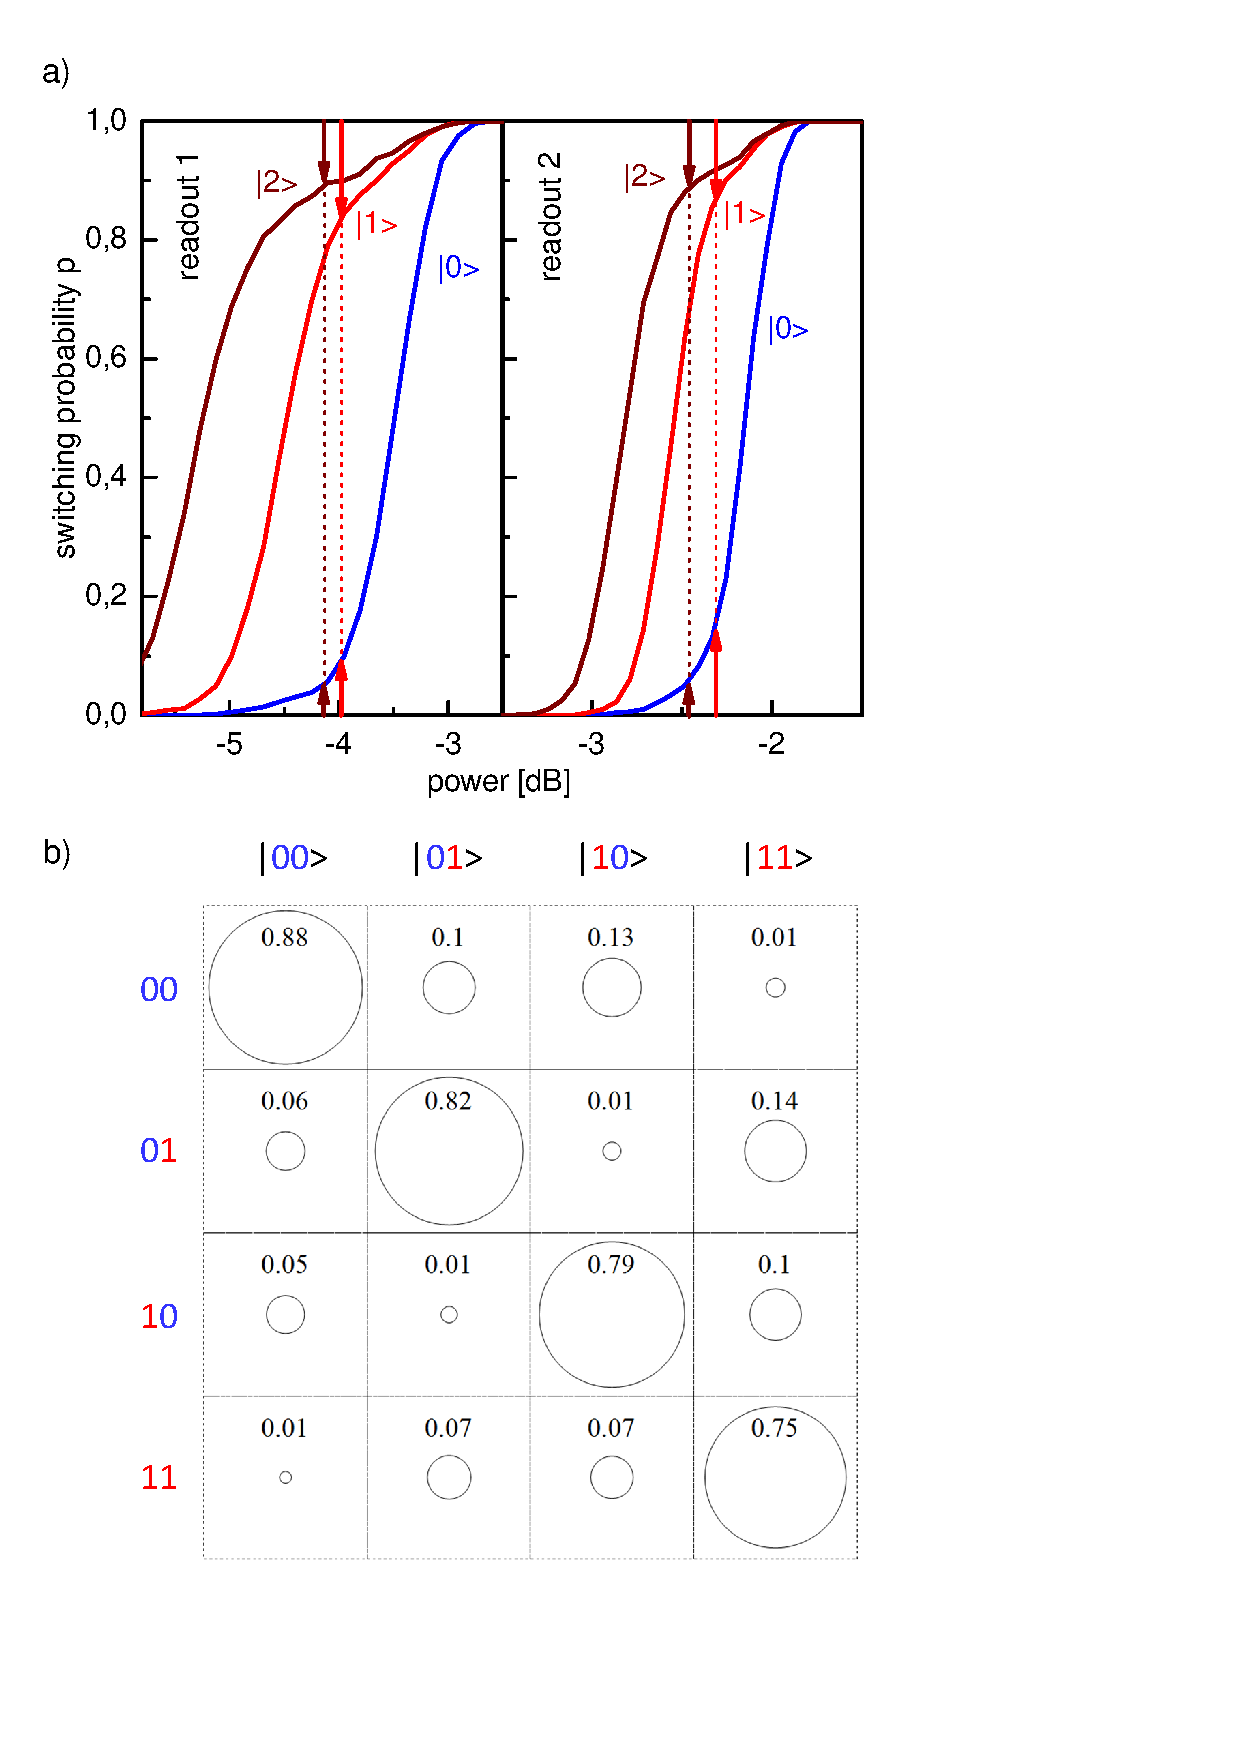
\includegraphics[width=8cm]{FigSuppl} \caption{\label{fig:readouterrors} }
(a) Switching probability $p$ of each readout as a function of its
peak driving power, when its qubit is prepared in state $\left|0\right\rangle $
(blue), $\left|1\right\rangle $ (red), or $\left|2\right\rangle $
(brown), with the other qubit being far detuned. The arrows indicate
the readout errors where the contrast is optimal with (brown) and
without (red) $\left|1\right\rangle \rightarrow\left|2\right\rangle $
shelving. (b) Readout matrix giving the probabilities of the four
$ab$ outcomes, for the four computational input states $|uv\rangle$,
when using $\left|1\right\rangle \rightarrow\left|2\right\rangle $
shelving. 
\end{figure}


Errors in our readout scheme are discussed in detail in {[}13{]} for
a single qubit. First, incorrect mapping $\left|0\right\rangle \rightarrow1$
or$\left|1\right\rangle \rightarrow0$ of the projected state of the
qubit to the dynamical state of the resonator can occur, due to the
stochastic nature of the switching between the two dynamical states.
As shown in Fig. S4.1, the probability $p$ to obtain the outcome
1 varies continuously from 0 to 1 over a certain range of drive power
$P_{\mathrm{d}}$ applied to the readout. When the shift in power
between the two $p_{\left|0\right\rangle ,\left|1\right\rangle }(P_{\mathrm{d}})$
curves is not much larger than this range, the two curves overlap
and errors are significant even at the optimal drive power where the
difference in $p$ is maximum. Second, even in the case of non overlapping
$p_{\left|0\right\rangle ,\left|1\right\rangle }(P_{\mathrm{d}})$
curves, the qubit initially projected in state$\left|1\right\rangle $
can relax down to $\left|0\right\rangle $ before the end of the measurement,
yielding an outcome 0 instead of 1. The probability of these two types
of errors vary in opposite directions as a function of the frequency
detuning $\Delta=\nu_{\mathrm{R}}-\nu>0$ between the resonator and
the qubit, so that a compromise has to be found for $\Delta$. As
explained in the main text, we use a shelving method to the second
excited state in order to improve the readout contrast $c=Max\left(p_{\left|1\right\rangle }-p_{\left|0\right\rangle }\right)$,
with a microwave $\pi$ pulse at frequency $\nu_{12}$ bringing state
$\left|1\right\rangle $ into state $\left|2\right\rangle $ just
before the readout pulse. The smallest errors $e_{0}^{\mathrm{I,II}}$
and $e_{1}^{\mathrm{I,II}}$ when reading $\left|0\right\rangle $
and $\left|1\right\rangle $ are found for $\Delta_{\mathrm{I}}=440\,\mathrm{MHz}$
and $\Delta_{\mathrm{II}}=575\,\mathrm{MHz}$: $e_{0}^{\mathrm{I}}=5\%$
and $e_{1}^{\mathrm{I}}=13\%$ (contrast $c_{\mathrm{I}}=1-e_{0}^{\mathrm{I}}-e_{1}^{\mathrm{I}}=82\%$),
and $e_{0}^{\mathrm{II}}=5.5\%$ and $e_{1}^{\mathrm{II}}=12\%$ ($c_{\mathrm{II}}=82\%$).
When using the $\left|1\right\rangle \rightarrow\left|2\right\rangle $
shelving before readout, $e_{0}^{\mathrm{I}}=2.5\%$ and $e_{2}^{\mathrm{I}}=9.5\%$
(contrast $c_{\mathrm{I}}==1-e_{0}^{\mathrm{I}}-e_{2}^{\mathrm{I}}=88\%$),
and $e_{0}^{\mathrm{II}}=3\%$ and $e_{2}^{\mathrm{II}}=8\%$ ($c_{\mathrm{II}}=89\%$).
These best results are very close to those obtained in {[}12{]}, but
cannot however be exploited for simultaneous readout of the two qubits.

Indeed, when the two qubits are measured simultaneously, we find an
influence of the projected state of each qubit on the outcome of the
readout of the other one. In order to to minimize this spurious effect,
we increase the detuning $\Delta_{\mathrm{I,II}}$ up to $\sim1\,\mathrm{GHz}$
with respect to previous optimal values. An immediate consequence
shown in Fig. S4.1(a) is a reduction of the $c_{\mathrm{I,II}}$ contrasts.
The errors when reading $\left|0\right\rangle $ and $\left|1\right\rangle $
are then $e_{0}^{\mathrm{I}}=10\,\%$ and $e_{1}^{\mathrm{I}}=16\,\%$
(contrast $c_{\mathrm{I}}=74\%$) and $e_{0}^{\mathrm{II}}=12\,\%$
and $e_{1}^{\mathrm{II}}=15\,\%$ (contrast $c_{\mathrm{II}}=73\%$).
When shelving the qubit in state $\left|2\right\rangle $ , the errors
are $e_{0}^{\mathrm{I}}=5\,\%$, $e_{2}^{\mathrm{I}}=11\,\%$ (contrast
$c_{\mathrm{I}}=84\%$), $e_{0}^{\mathrm{II}}=5\,\%$, $e_{2}^{\mathrm{II}}=12\,\%$
(contrast $c_{\mathrm{I}}=83\%$). The readout errors are captured
in the $4\times4$ readout matrix $\mathcal{R}$ shown in Fig. S4.1(c),
that gives the probabilities $p_{\mathrm{uv}}$ of the four possible
outcomes for the different input states using the $\left|1\right\rangle \rightarrow\left|2\right\rangle $
shelving technique. This matrix $\mathcal{R}$ is used to correct
the readout errors only when doing state tomography, and not when
the running the algorithm once. The cause of the readout crosstalk
in our processor is discussed in {[}11{]}.


\paragraph{S5. Algorithm Fidelity\protect \\
}

The fidelity of each possible outcome $ab$ $\in\{00,01,10,11\}$
of our algorithm is given as \[
f_{ab}=p_{ab/|ab\rangle}/\left(p_{ab/|00\rangle}+p_{ab/|01\rangle}+p_{ab/|10\rangle}+p_{ab/|11\rangle}\right),\]
where $p_{ab/|uv\rangle}$ is the conditional probability for obtaining
$ab$ when the state $|uv\rangle$ has been marked by the oracle $O_{uv}$.
Table \ref{tab:Probabilities-for-obtaining} shows these probabilities
$p_{ab/|uv\rangle}$ for all possible combinations of $ab$ and $|uv\rangle$
as well as the fidelities $f_{ab}$. The average fidelity of the algorithm
is 59.1 \%.

%
\begin{table}[H]
\begin{centering}
\begin{tabular}{|c|c|c|c|c|c|c|}
\hline 
$ab$/$|uv\rangle$ & $\left|00\right\rangle $ & $\left|01\right\rangle $ & $\left|10\right\rangle $ & $\left|11\right\rangle $ & $\sum$ & $f_{ab}$\tabularnewline
\hline
\hline 
00 & 0.666 & 0.192 & 0.188 & 0.122 & 1.168 & 57.0 \%\tabularnewline
\hline 
01 & 0.127 & 0.554 & 0.071 & 0.122 & 0.874 & 63.4 \%\tabularnewline
\hline 
10 & 0.128 & 0.106 & 0.615 & 0.239 & 1.088 & 56.5 \%\tabularnewline
\hline 
11 & 0.079 & 0.148 & 0.126 & 0.517 & 0.870 & 59.4 \%\tabularnewline
\hline
\end{tabular}
\par\end{centering}

\caption{\label{tab:Probabilities-for-obtaining}Conditional probabilities
$p_{ab/|uv\rangle}$ and statistical fidelities $f_{ab}$ for all
possible outcomes $ab$, measured for our version of Grover's algorithm.}

\end{table}

\begin{thebibliography}{1}
\bibitem{FlorianKerr} F. R. Ong \textit{et al.}, Phys. Rev. Lett.
106, 167002 (2011).
\end{thebibliography}

\end{document}
